\section{La page des tournois}

\begin{figure}[H]
\centering
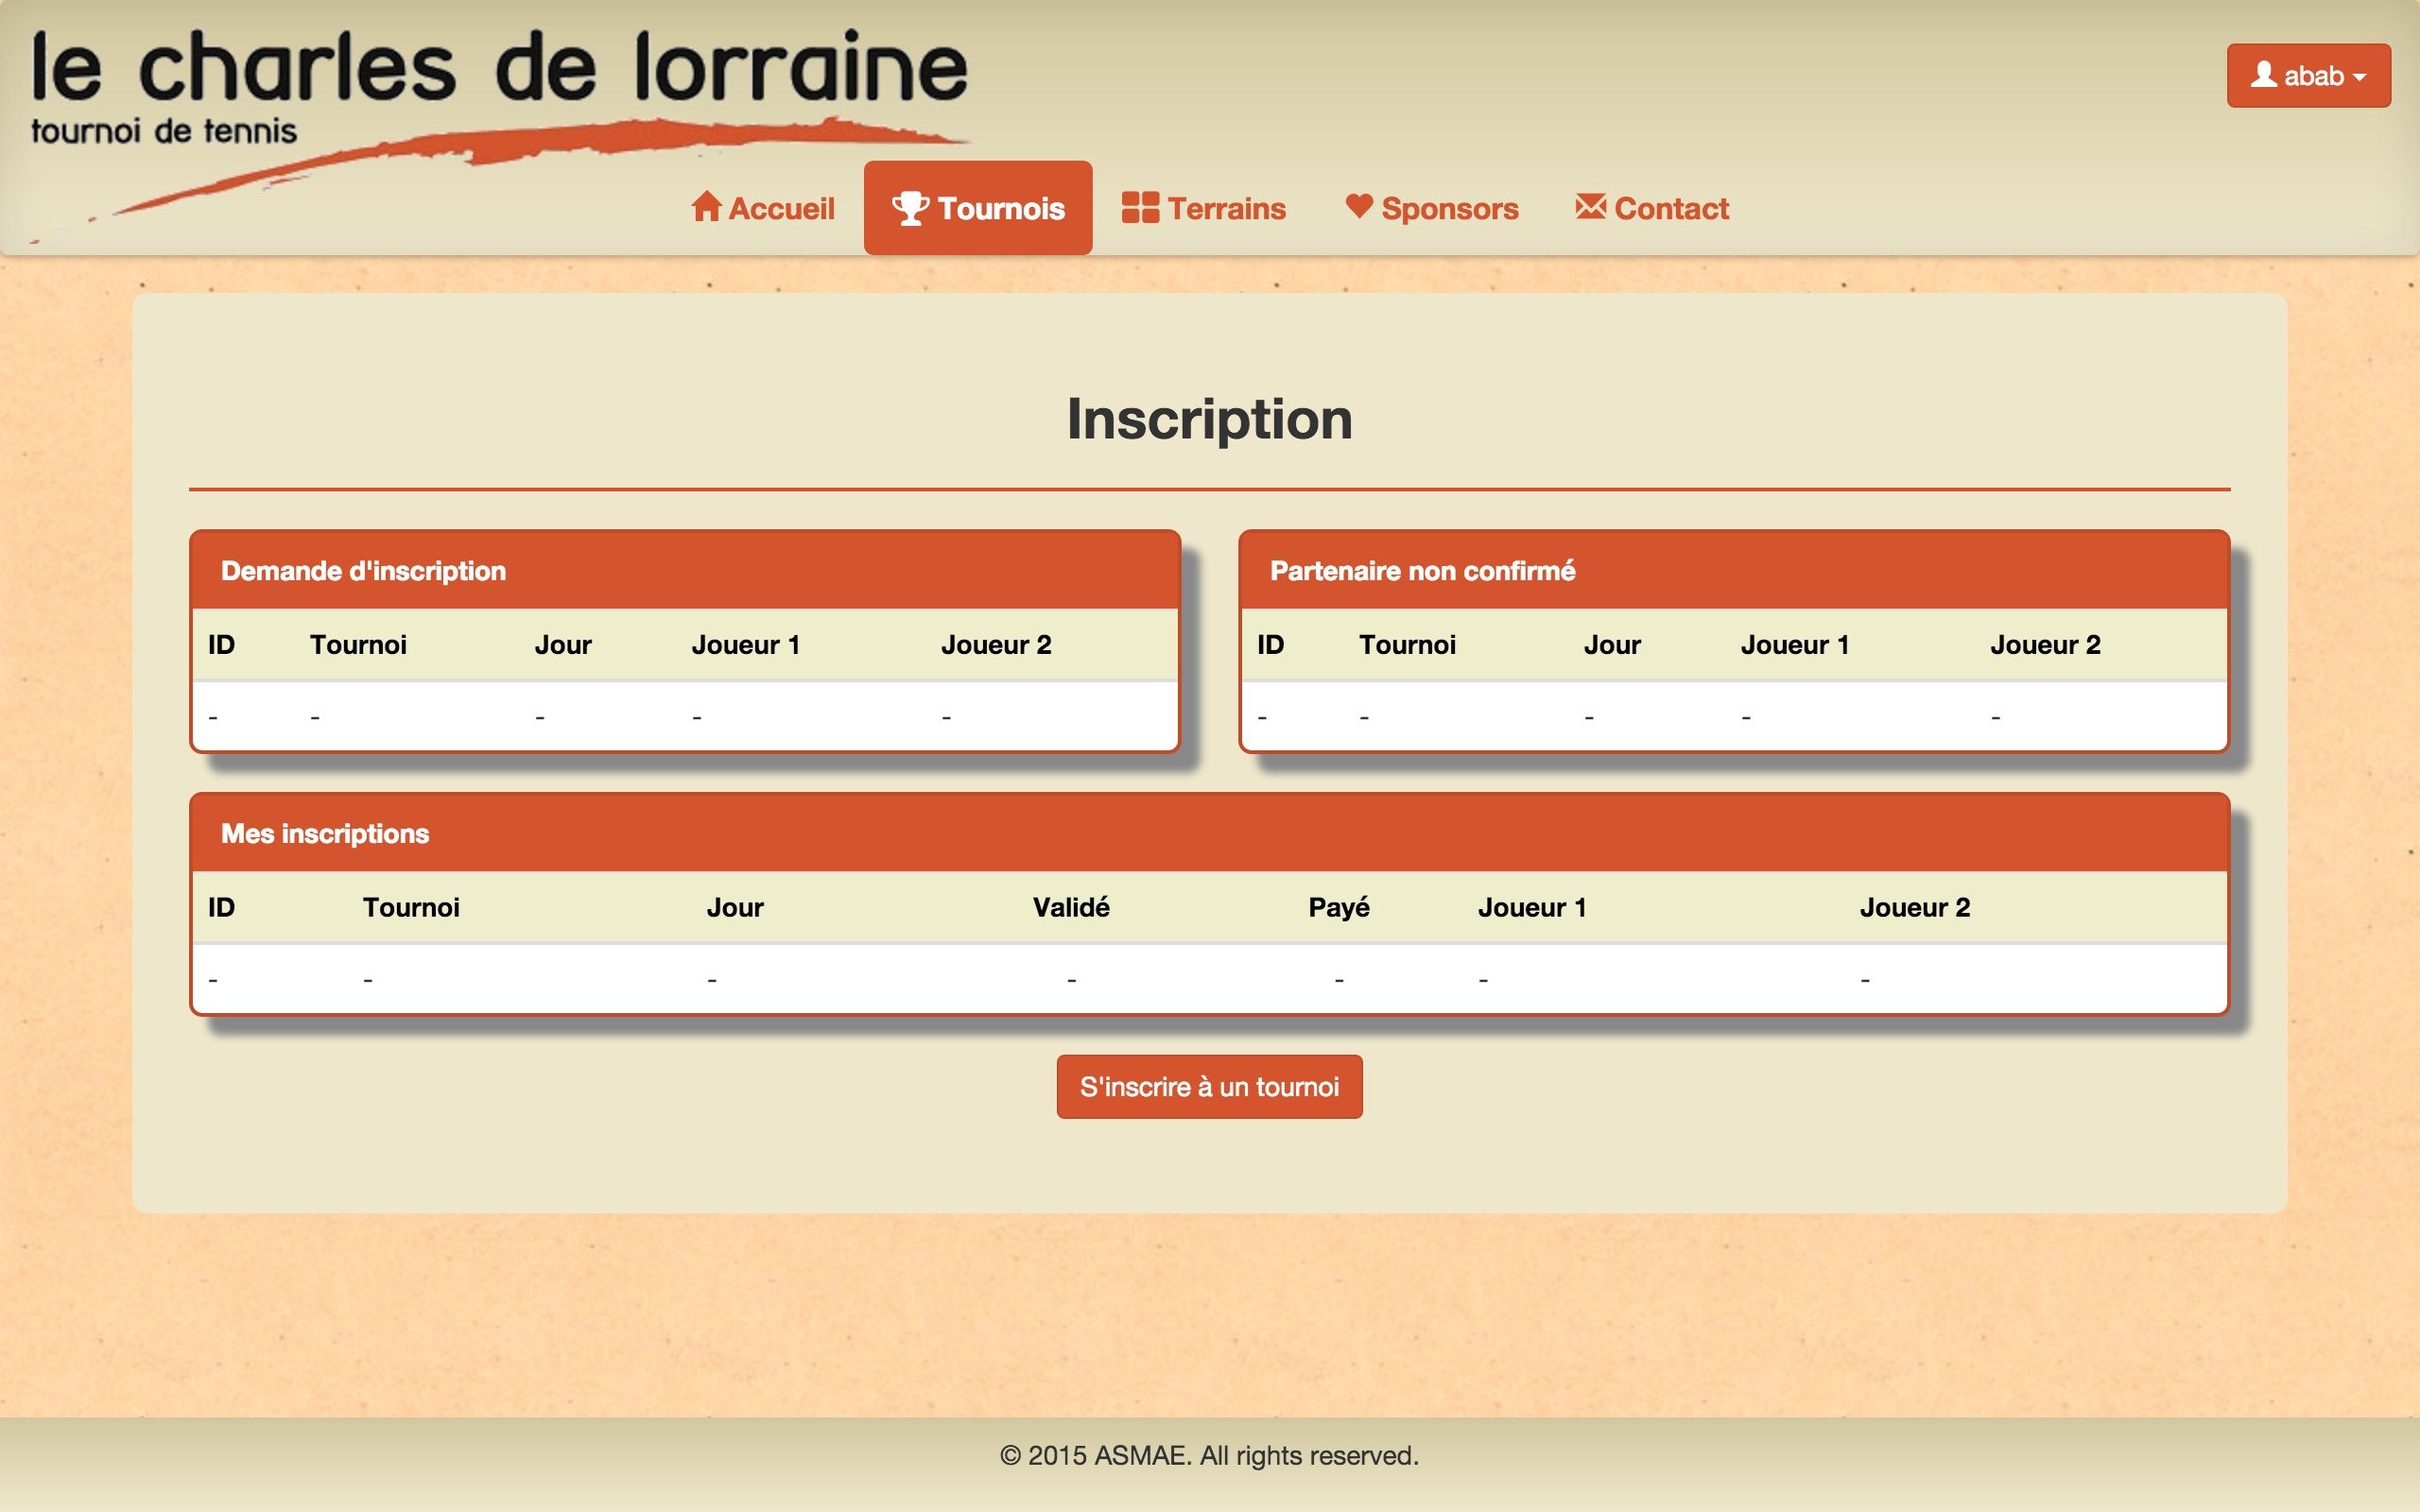
\includegraphics[scale=0.15]{page-tournois/page-tournois.jpg}
\caption{Page des tournois}
\end{figure}

\subsection{Vos inscriptions}

Depuis la page \enquote{Tournois}, vous pouvez gérer vos inscriptions. \newline

Il y a 3 catégories d'inscription : \newline

\begin{description}
    \item[Les demandes d'inscription] : elles émanent d'autres joueurs qui
    vous proposent de former une paire, vous pouvez cliquer dessus, faire vos
    choix et indiquer des commentaires supplémentaires pour l'équipe et ensuite
    valider ; ou vous pouvez refuser la demande du joueur.
    \item[Les partenaires non confirmés] : ce sont les demandes que vous avez
    faites à d'autres joueurs et qui sont en attente de confirmation de sa part.
    Si vous ne souhaitez plus proposer à l'autre joueur de former une paire,
    vous pouvez supprimer votre demande en cliquant dessus et en appuyant sur
    \textit{Supprimer}.
    \item[Les inscriptions confirmées] : elles signifient que vous et votre
    partenaire avez accepté de former une paire. Vous pouvez cliquer dessus
    pour voir un résumé de votre demande et effectuer votre paiement.
\end{description}
